\documentclass[11pt]{article}

%\documentclass[11 pt]{article}
\usepackage{graphicx}
\usepackage{float}
\usepackage{tabularx,ragged2e}
\usepackage{siunitx}
\usepackage{listings}


\usepackage{rotating}
\usepackage[utf8]{inputenc}

\usepackage[square,sort,comma,numbers]{natbib}
\bibliographystyle{abbrvnat}
\setcitestyle{authoryear,open={(},close={)}} %Citation-related commands

\usepackage{setspace}\doublespacing
\usepackage[dvipsnames]{xcolor}
\usepackage{lineno}
\linenumbers
\usepackage[normalem]{ulem} 
\usepackage{multicol}
\usepackage{hyperref}
\hypersetup{
	colorlinks=false,
%	linkcolor=blue,
%	filecolor=magenta,      
%	urlcolor=cyan,
	pdftitle={Overleaf Example},
	pdfpagemode=FullScreen,
}

\addtolength{\oddsidemargin}{-2.5cm}
\addtolength{\evensidemargin}{-1.5cm}

\addtolength{\textwidth}{5.5cm}

\addtolength{\topmargin}{-.875in}
\addtolength{\textheight}{1.75in}

%\author{Pending}

\begin{document}
\begin{flushright}
%    MBE - Methods article
\end{flushright}
\begin{center}
	\begin{LARGE}
		\textbf{Untangling temporal signal and the phylodynamic threshold of microbial sequence data sets}
	\end{LARGE}
	
	John H Tay$^1$, Sebastian Duchene$^{1, 2*}$.

$^1$Peter Doherty Institute for Infection and Immunity, Department of Microbiology and Immunology, University of Melbourne, Melbourne, Australia.

$^2$Department of Computational Biology, Institut Pasteur, Paris, France.

\end{center}
*email: sduchene@pasteur.fr

\begin{Large}
	\textbf{Abstract} ($\le$300 words)
\end{Large}
Our understanding of the evolution of many microbes has been revolutionised by the molecular clock, a statistical tool to infer evolutionary rates and timescales. The fundamental assumption of molecular clock models is that the rate at which substitutions accumulate can be described by a statistical process. In all molecular clock models evolutionary rates and times are unidentifiable, and therefore 'calibration' information is essential to obtain estimates in calendar time.

For many microbes, the sequence sampling times themselves can be often used for calibration. Phylogenetic tests of temporal signal are often used to decide whether such calibrations are reliable. Critically, in addition to the calibration information, the full Bayesian phylogenetic model also includes the molecular clock model and a branching process (tree prior). As a result, there are multiple sources of information that are difficult to untangle.

We assessed temporal signal in three microbial data sets of human and animal diseases with a range of evolutionary characteristics and with ancient DNA sequences; \textit{Powassan virus} (POWV), the cholera bacetrium (\textit{Vibrio cholerae}), and the syphilis bacterium (\textit{Treponema palladium.}). We found that the tree prior can have a substantial impact on whether temporal signal is detected. To investigate this problem we conducted extensive simulations and calculated the sensitivity and specificity of these tests under several tree priors. 

We find that highly informative sequence data sets are generally robust to the tree prior. In contrast, in data sets with low information content, choosing a prior that is highly informative and inconsistent with the data can result in the false rejection of temporal signal. 

We propose prior sensitivity analyses and prior predictive simulations to determine whether the prior is reasonable and to improve the detection of temporal signal and maximise the information that can be drawn from molecular sequence data sets.

\textbf{Key words:} Molecular clock, Ancient DNA, Bayesian phylogenetics, Microbial evolution.

\section{Introduction}
Molecular sequence data have been essential to unravel the evolutionary history of many organisms. The molecular clock is a statistical tool that posits that molecular evolution, in the form of substitutions, follows a statistical process. For example, under the simplest molecular clock model, known as the strict clock, substitutions accumulate linearly over time along a lineage, such that the evolutionary rate is constant over time \citep{zuckerkandl1965evolutionary}. At the other end of the spectrum, relaxed molecular clocks allow every lineage in a phylogenetic tree to display a different evolutionary rate (\cite{drummond2006relaxed} and reviewed in \citep{ho2014molecular}). 

All molecular clock models have a fundamental limitation, where evolutionary rates and times are unidentifiable. That is, there exist an infinite number of combinations of evolutionary rates and times that are compatible with an amount of evolutionary divergence \cite{yang2006bayesian,dos2013unbearable}. For this reason, external information, known as a molecular clock calibration is necessary to produce estimates in calendar units. As a case in point, consider two sequences whose genetic divergence from their most recent common ancestor is 10 subs/site. In the absence of calibrating information it is impossible to know \texit{how rapidly} they evolve and \texit{when} they diverged. The calibration can be a known evolutionary rate, such as 1 subs/site/year, or a divergence date, such as 1 year before present. The genetic distance can be divided by the evolutionary rate to infer the divergence time to infer a time to the most recent common ancestor of 10 years, or the genetic distance can be divided by the divergence date to infer the evolutionary rate, 10/subs/site/year in this case.

The finding that some organisms accumulate substitutions in a measurable timescale prompted the use of sequence sampling times for calibration \citep{drummond2003measurably}. The motivation behind this practice is that sequence data collected at different points in time would have accumulated a corresponding number of substitutions. With the example above, a sequence collected six months of the common ancestor would have accumulated 5 subs/site (10 subs/site/year $\times$ 0.5 years = 5 subs/site), whereas one collected after 1 year would have accrued 10 subs/site (10 subs/site/year$\times$ 1 year = 10 subs/site). As a result, sequence sampling times act as a time-calibration that is intuitively informative about the evolutionary rate.

A fundamental question to warrant the use of sampling times for molecular calibration is the extent to which a data set behaves as a measurably evolving population. 

\textbf{Outline}

\textbf{\textcolor{blue}{Key points for Results section - 28 / 02 / 2024}}
\begin{itemize}
	\item The impact of the tree prior and hyperpriors on model selection. Here show the polygons and tables. Pow is particularly interesting because the exponential prior on $\Phi$ does not support temporal signal. \textbf{Result: Priors obviously impact marginal   likelihoods, but sometimes also model choice.}
        \subitem \textcolor{red}{To do: Make figure with polygons for all data sets, add legends, etc... Also make latex table with marginal likelihoods, but only those that have sufficient ESS.}
        \begin{center}
            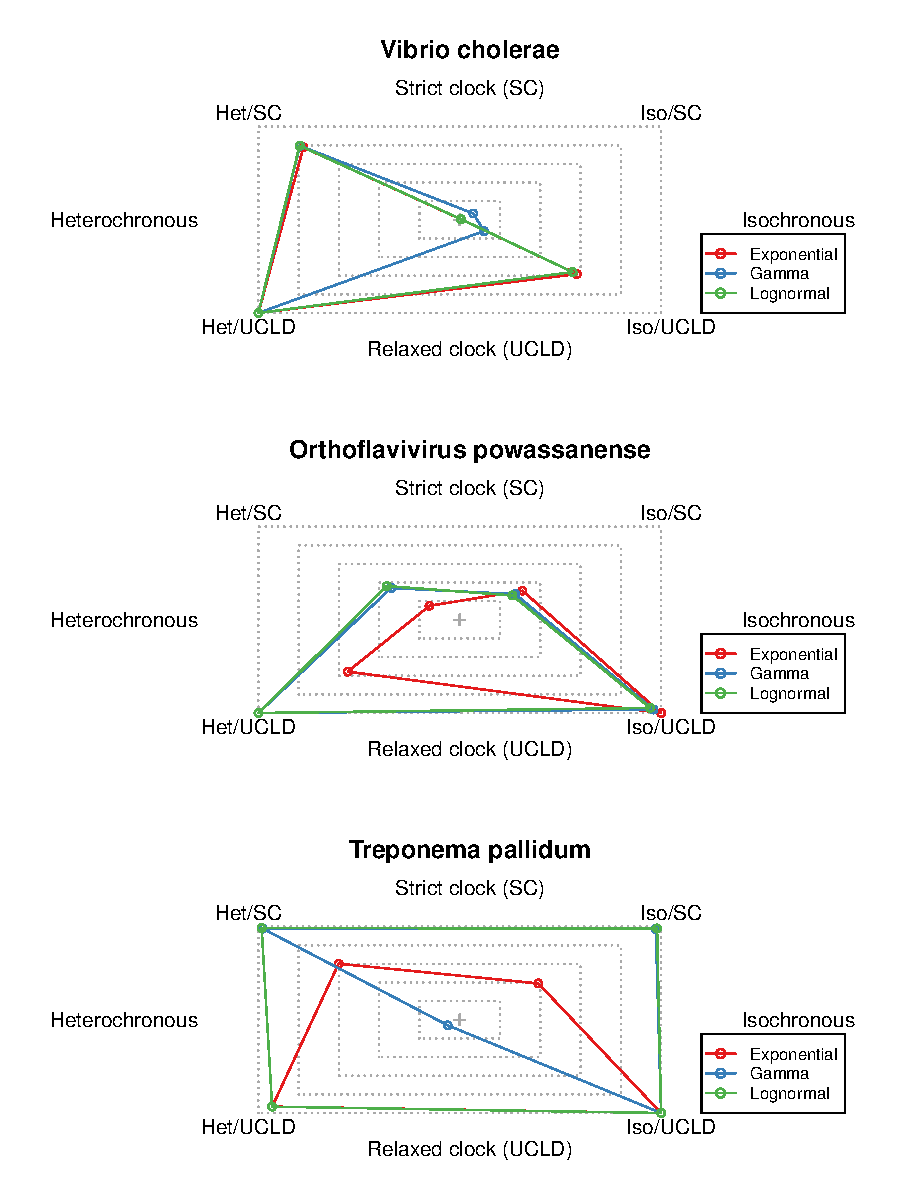
\includegraphics[width=14cm]{sandbox_figures/polygon_plot.pdf}\newline
            A polygon plot of the relative log marginal likelihoods of each microbe dataset under a different population size prior, analysed with four different configurations. Het (heterochronous) includes sampling, while iso (isochronous) does not include any sampling times. SC is strict clock and UCLD is the uncorrelated lognormal relaxed clock. Red represents an exponential hyperprior on the population size, blue is a gamma hyperprior, and green is a lognormal hyperprior.
        \end{center}
        \begin{table}[H]
        \caption{Log Bayes factors between isochronous and heterochronous models for each dataset, separated by prior on population size}
        \begin{center}
        \begin{tabular}{ c | c c c }
         & Exponential & Gamma & Lognormal \\ 
        \hline
        Vibrio cholerae; Strict Clock & 355.18 & 379.63 & 382.10 \\  Lorem ipsum dolor sit~\cite{bib1} amet, consectetur adipiscing elit. Curabitur eget porta erat. Morbi consectetur est vel gravida pretium. Suspendisse ut dui eu ante cursus gravida non sed sem. Nullam Eq~(\ref{eq:schemeP}) sapien tellus, commodo id velit id, eleifend volutpat quam. Phasellus mauris velit, dapibus finibus elementum vel, pulvinar non tellus. Nunc pellentesque pretium diam, quis maximus dolor faucibus id.~\cite{bib2} Nunc convallis sodales ante, ut ullamcorper est egestas vitae. Nam sit amet enim ultrices, ultrices elit pulvinar, volutpat risus.
        Vibrio cholerae; Relaxed Clock & 208.97 & 439.63 & 219.60 \\   
        Orthoflavivirus powassanense; Strict Clock & -80.63 & 32.67 & 50.29 \\  
        Orthoflavivirus powassanense; Relaxed Clock & -221.94 & 18.79  & 27.23 \\   
        Treponema pallidum; Strict Clock & 105.80 & 2.17 & 1.85 \\  
        Treponema pallidum; Relaxed Clock & -34.37 & -1474.14 & -34.04
        \end{tabular}n
        \end{center}
        \end{table}
    
	\item Show clock rate (ucld.mean and clock.rate), root height, tree length, and coefficient of rate variation (only for the relaxed clock) distributions under each clock model and prior. \textbf{Result: Estimates of evolutionary rates and times are generally robust to the tree prior even if the marginal likelihood is not}
        \subitem \textcolor{red}{To do: Plot densities of clock rates, root height, tree length, coefficient of rate variation. One panel per data set, show density for the three priors and the same colours as the fig above.}
        \begin{center}
            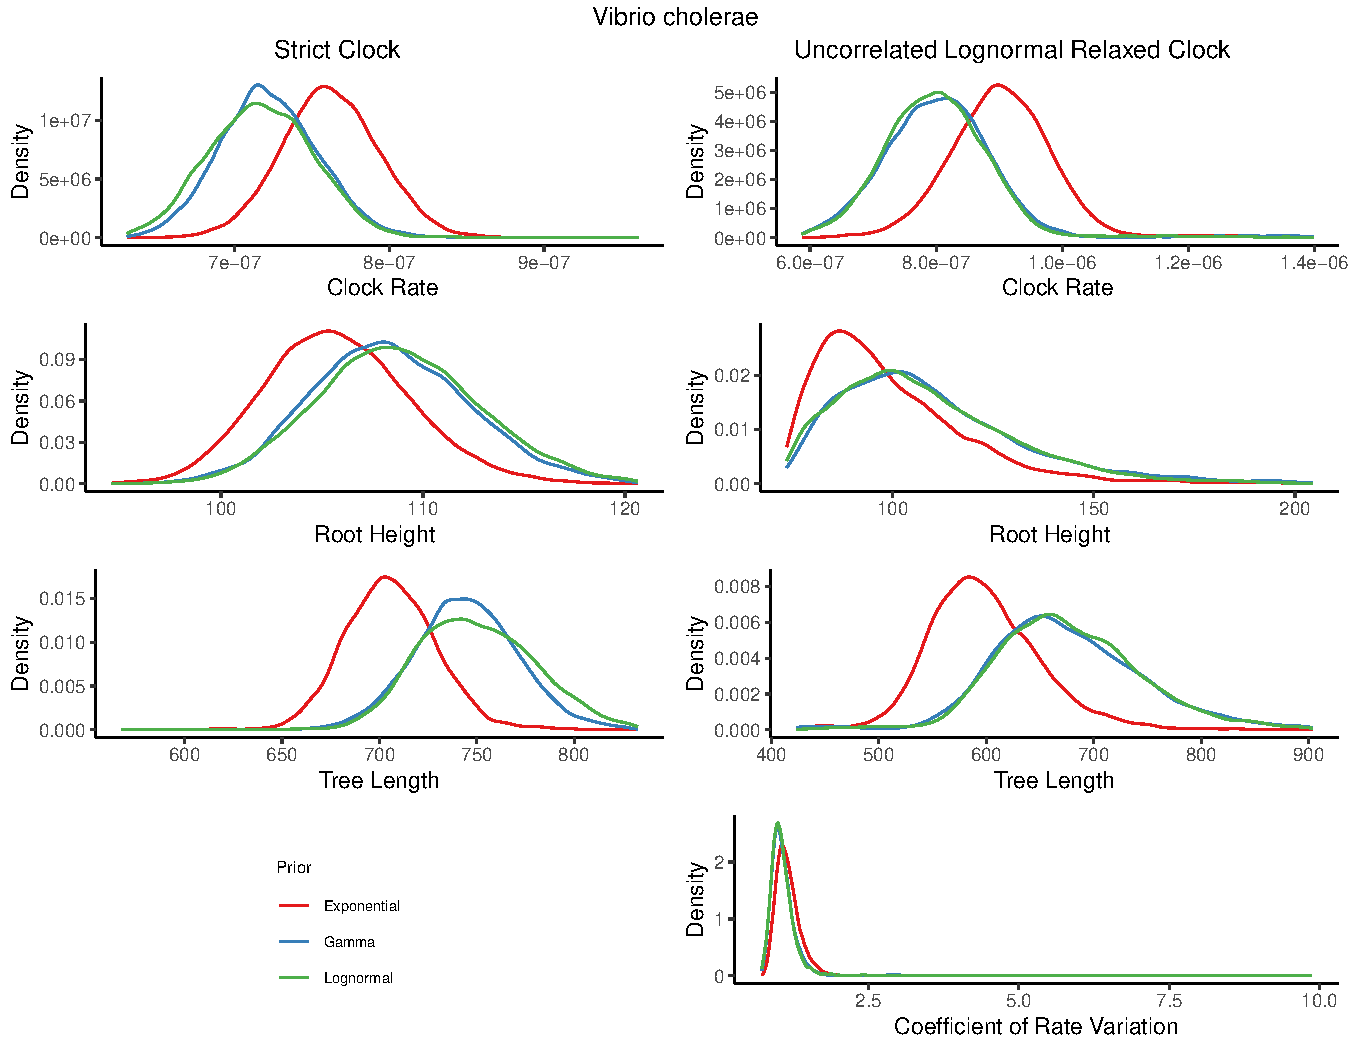
\includegraphics[width=17cm]{sandbox_figures/cholera_density_plot.pdf}\newline
            Density plots of the clock rate, root height, tree length, and coeffcient of rate variation of cholera.
            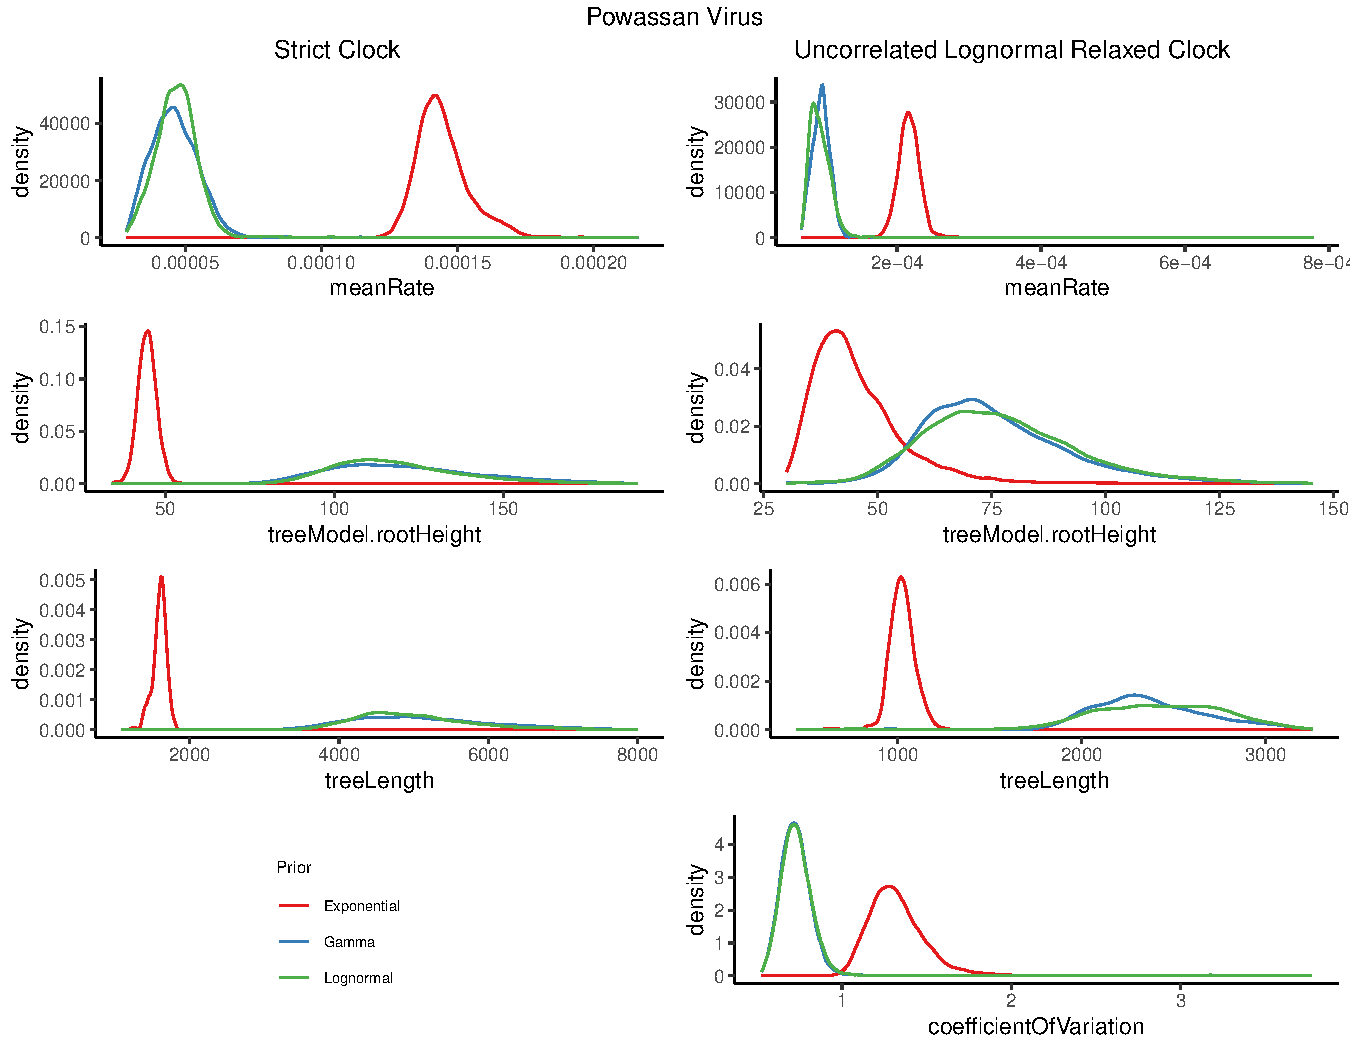
\includegraphics[width=17cm]{sandbox_figures/powv_density_plot.pdf}\newline
            Density plots of the clock rate, root height, tree length, and coeffcient of rate variation of powassan virus.
            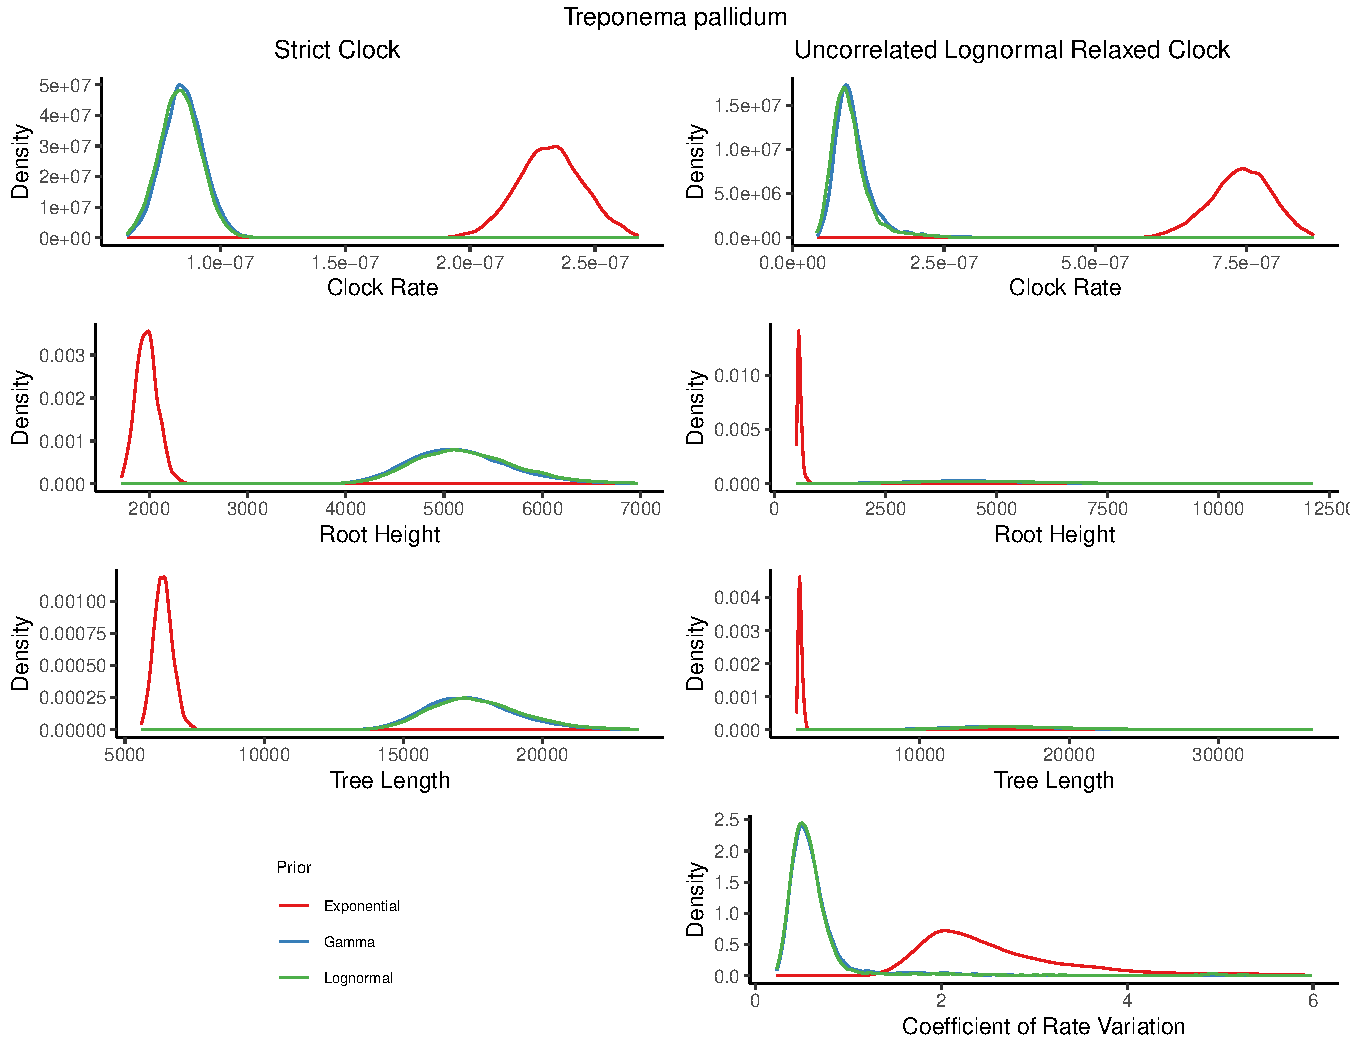
\includegraphics[width=17cm]{sandbox_figures/treponema_density_plot.pdf}\newline
            Density plots of the clock rate, root height, tree length, and coeffcient of rate variation of treponema palladium.
        \end{center}
	
    \item Simulations \textbf{\textcolor{red}{Pending for now} - does the tree prior impact the accuracy to detect temporal signal?}
        \subitem \textcolor{red}{To do: This is where the simulations come in. Think of visuals here. Probably best displayed as tables? We can also just have plots of error bars per analysis to show coverage of key parameters...}
        \begin{table}[H]
        \caption{Heterochronous}
        \begin{center}
        \begin{tabular}{ c | c c c }
         & Exponential & Gamma & Lognormal \\ 
        \hline
        Vibrio cholerae; Strict Clock & 1.0 & 1.0 & 1.0 \\  
        Vibrio cholerae; Relaxed Clock &  &  &  \\   
        Orthoflavivirus powassanense; Strict Clock &  &  &  \\  
        Orthoflavivirus powassanense; Relaxed Clock &  &  &  \\   
        Treponema pallidum; Strict Clock & 0.0 & 0.0 & 0.0 \\  
        Treponema pallidum; Relaxed Clock &  &  & 
        \end{tabular}
        \end{center}
        \end{table}

        \begin{table}[H]
        \caption{Isochronous}
        \begin{center}
        \begin{tabular}{ c | c c c }
         & Exponential & Gamma & Lognormal \\ 
        \hline
        Vibrio cholerae; Strict Clock & .0 & .0 & .0 \\  
        Vibrio cholerae; Relaxed Clock &  &  &  \\   
        Orthoflavivirus powassanense; Strict Clock &  &  &  \\  
        Orthoflavivirus powassanense; Relaxed Clock &  &  &  \\   
        Treponema pallidum; Strict Clock & .0 & .0 & .0 \\  
        Treponema pallidum; Relaxed Clock &  &  & 
        \end{tabular}
        \end{center}
        \end{table}
    
	\item Why does the prior on $\Phi$ impact temporal signal? Because it is linked to tree length and to the clock rate via the coalescent and the CTMC reference prior. Here show pairs plots for the root height, $\Phi$, tree length, clock rate \textbf{Result: Some parameters in the Bayesian hierarchical model are naturally correlated, the marginal prior is not obvious, but can be easily inspected}
            \subitem \textcolor{red}{To do: we should do pairwise plots to show the association of the parameters above ($\Phi$, tree length, tree height, clock rate). This is just sampling from the prior, which I have done. Can we do this for the three priors on $\Phi$, using the colours above?}   
        
	\item Inspecting the marginal prior is important and should be conducted prior to tests of temporal signal. For example, including monophyletic constraints, and other prior information can impact temporal signal. 
	\item Prior sensitivity is also important to assess the robustness of the estimates.
 
\end{itemize}

\Large{\textbf{\textcolor{blue}{General outline and key points}}}

\begin{itemize}
	\item Talk about tests of temporal signal
	\item The role of BETS
	\item pitfals of BETS: that we don't know the effect of the tree prior, all priors should be proper, impact of the clock model (because it can absorb rate variation among lineages).
	\item introduce data sets
	\item analyses of empirical data
	\subitem Use constant coalescent with the three population size priors and explain that they result in different priors on the clock rate and on the tree height. What are the implications here?
	\subitem Use the skyride and show the marginal prior on clock rate and tree height.
	\item Simulations. We should only do these for the best fitting model clock model per data set. But here, let's stick to the constant-size coalescent because it is more practical. 
	\subitem How well do they classify data sets as having temporal signal? think about error rates.
	\subitem Does the classification accuracy depend on the average logBFs for those data sets that do have temporal signal? What I mean here is that the cholera ones would naturally have stronger temporal signal than the treponema ones, so we expect different error rates. 
	\item Conclude: What is the best strategy here regarding tree prior? comment on the clock prior? where doe the regression fit in here? what about prior and posterior predictive checks?
\end{itemize}

\begin{itemize}
	\item What does the root height, tree length, and clock rate prior look in each case (coalescent with all priors, skyride)?
	\subitem How do these priors impact the phylogenetic likelihood? The point here is that if the tree prior is very wrong (i.e. it is in conflict with the likelihood) then it can mislead tests of temporal signal.
	\subitem with the relaxed clock it is useful to inspect whether the coefficient of rate variation is larger
	\item Ideally the test should assess only the sampling times
	
\end{itemize}



\textbf{Prior sensitivity to run (21 Feb)}
\begin{itemize}
	\item Run all three priors on $\Phi$ and check
	\subitem tree height, clock rate, tree length, pop size - and correlations
	\item Run with a set of fixed $\Phi$ values and show how the mean and variance of clock rate, tree height and tree length changes 
\end{itemize}

\textbf{new results, as of 12 Feb}
\begin{itemize}
	\item The prior on the population size seems to matter when we don't have temporal signal. It tends to lead to false positives. 
	\item A data set with temporal signal, will generally be robust to the prior. 
	\item Redefine temporal signal. It is when the data are more informative than the prior in a Bayesian context.
	\item But this is not a problem in itself. One should choose a prior that is sensible. Some data sets, like cholera will be robust to the choice of prior. They are more informative and have stronger temporal signal. 
\end{itemize}





\begin{Large}
	\textbf{Introduction}
\end{Large}

Pending


\begin{table}[H]
\caption{Proportion of simulations with temporal signal according to log Bayes factors support (log BF)}
\begin{center} 
	\label{table:logBF_pp_correspondence}
	\begin{tabular}{c|c|c|c|c}
		Prior on $\Phi$ and clock model & $log BF\ge0$ & $log BF\ge1$ & $log BF\ge3$ & $log BF\ge5$\\
		\hline
		$\Gamma(\kappa=0.001, \theta=1000)$; SC & 0.25 & 0.23 & 0.21 & 0.21 \\
		$Lnorm(\mu=1.0, \sigma=5)$; SC & 0.42 & 0.40 & 0.33 & 0.26 \\
		$Exp(\mu=1.0)$; SC & NA & NA & NA & NA \\
	\end{tabular}
\end{center}	\vspace{-0.4cm}
\end{table}


\begin{figure}[H]
	\begin{center}
		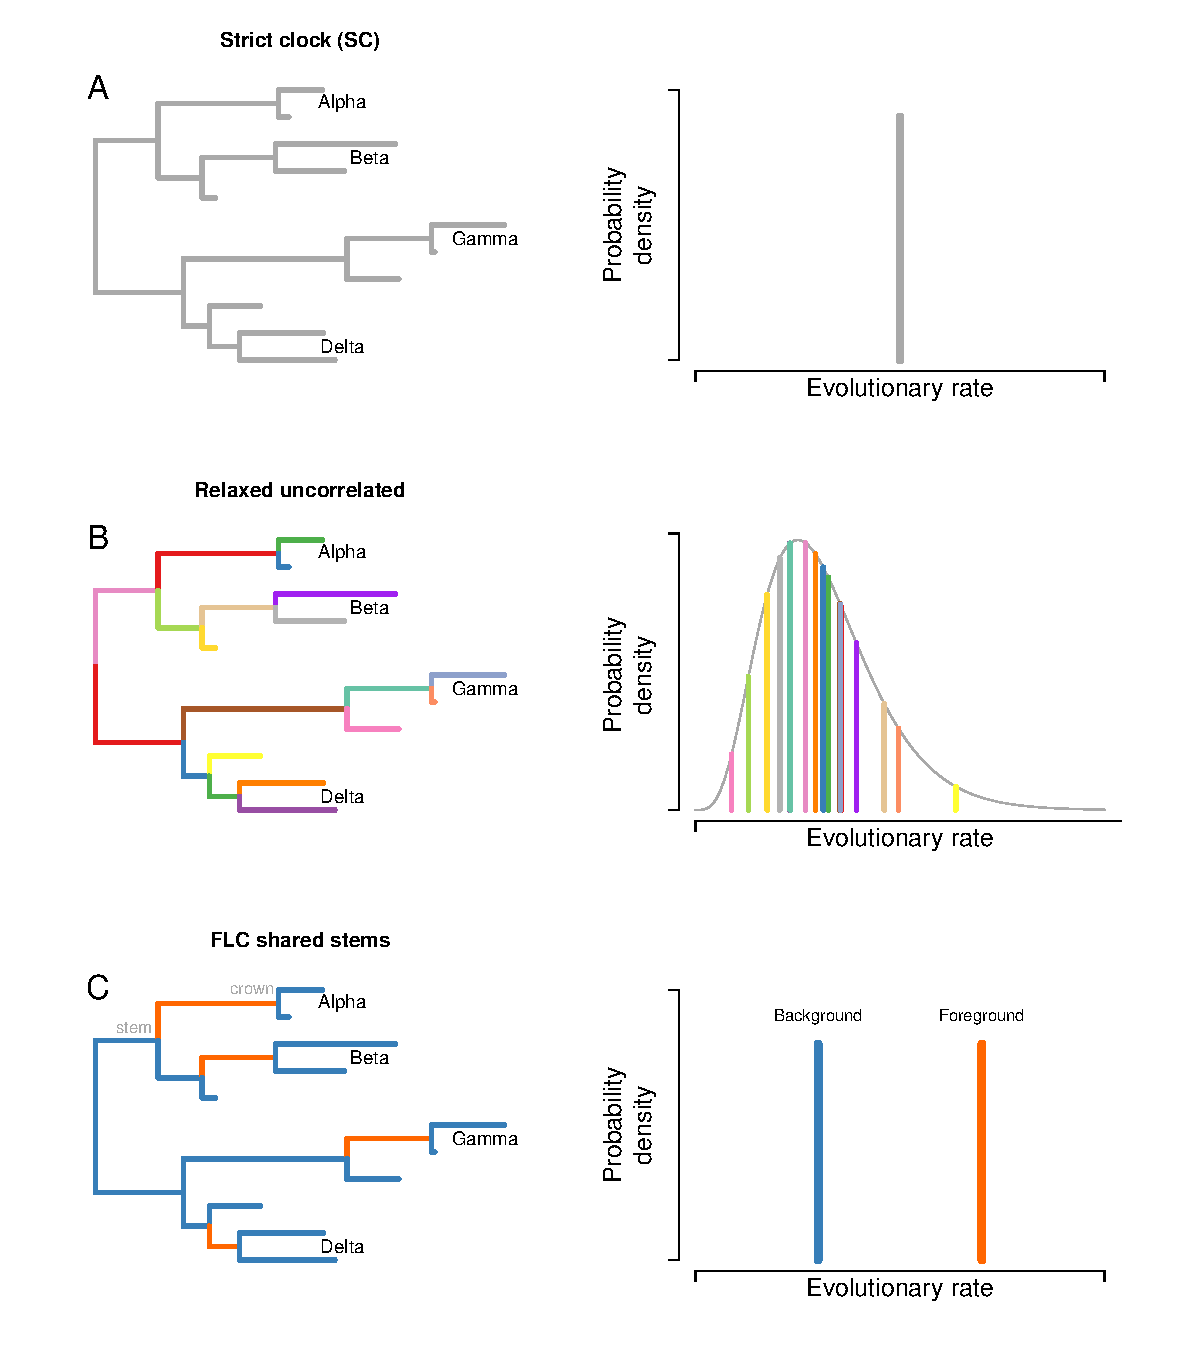
\includegraphics[width=17cm]{figures/clocks.pdf}% script: ternary_and_clock_plots.R
		\vspace{-0.5cm}
		\caption{Examples of molecular clock models. A. is a strict clock model (SC), where all branches share a single evolutionary rate. B. is an uncorrelated relaxed clock model, in which the evolutionary rates across branches are independent draws from an underlying statistical distribution, such as a lognormal or a gamma ($\Gamma$) distribution (typically abbreviated as UCLD and UCGD, respectively). Note that branches are coloured according to those drawn from the distribution on the right. C. represents a fixed local clock model, where stem branches leading up to variants of concern (VOCs; those leading to clades labelled as Alpha, Beta, Gamma and Delta, following variant names) are designated as the `foreground' and assigned a rate that differs from the `background'. In C, we have labelled the stem and crown nodes of variant Alpha, where evolutionary rate changes would have occurred.}
		\label{figure:clock_models}
	\end{center}
\end{figure}


\section{Supplementary Material}
Supplementary data are available at Molecular Biology and Evolution online.

\section{Acknowledgements}
The Authors thank two anonymous reviewers and the Editor for helpful comments in earlier versions of this manuscript. 

JHT and SD were supported by the Australian Research Council (FT220100629) and the Australian National Health and Medical Research Council (grant number 2017284). GB acknowledges support from the Internal Funds KU Leuven under grant agreement C14/18/094 and from the Research Foundation -- Flanders (`Fonds voor Wetenschappelijk Onderzoek -- Vlaanderen', G0E1420N and G098321N).
The authors acknowledge efforts by originating and submitting laboratories for the sequence data in GISAID EpiCoV on which our empirical analyses are based. This research was undertaken using the LIEF HPC-GPGPU Facility hosted at the University of Melbourne. This Facility was established with the assistance of LIEF Grant LE170100200. 

\section{Data availability}
The data underlying this article are available in GISAID at gisaid.org, and all accession numbers are provided in Supplementary Material online.

%\bibliographystyle{plain}
\bibliography{References}

\end{document}
